%!TEX program = xelatex

% 纸张模式:护眼模式-geye 朦胧模式-hazy
% 纸张尺寸:pad kindle pc normal screen
\documentclass[cn, blue, normal, 12pt]{elegantnote}

\title{自动控制原理笔记}
\author{Xiaohei}
\version{1.2}
\date{\zhtoday}

\usepackage{pgfplots}
\pgfplotsset{compat=newest}
\usetikzlibrary{plotmarks}
\usetikzlibrary{arrows.meta}
\usepgfplotslibrary{patchplots}
\usepackage{grffile}
\usepackage{amsmath}
\usepackage{bm}
\usepackage{multirow}
\usepackage{yhmath}

\begin{document}

\setlength{\lineskip}{0}
\setlength{\parskip}{0}

\maketitle

\section{控制系统的数学模型}

\subsection{线性控制系统}

\textbf{线性控制系统描述方法}

\begin{enumerate}
    \item 输入输出描述法(外部描述法):输入输出模型
    \item 状态空间描述法(内部描述法):状态空间模型
\end{enumerate}

\textbf{线性控制系统输入输出数学模型}

\begin{enumerate}
    \item 时域模型:微分方程
    \item 频域、复频域模型:传递函数
    \item 图示模型:方框图、信号流图
\end{enumerate}

\subsection{典型环节}

\subsubsection{惯性环节}

\begin{equation}
    G(s)=\frac{1}{Ts+1}
\end{equation}

其中$T$为惯性环节时间常数。

\subsubsection{积分环节}

\begin{equation}
    G(s)=\frac{1}{Ts}
\end{equation}

其中$T$为积分环节时间常数。

\subsubsection{振荡环节}

\begin{equation}
    G(s)=\frac{\omega_n^2}{s^2+2\zeta\omega_n s+\omega_n^2}=\frac{1}{T^2 s^2+2\zeta Ts+1}
\end{equation}

其中$T=\frac{1}{\omega_n}$为时间常数,$\zeta$为阻尼比,$\omega_n$为无阻尼自然振荡角频率。

\subsubsection{微分环节}

\begin{equation}
    G(s)=Ts
\end{equation}

其中$T$为微分环节时间常数。理想微分环节的传递函数不是真有理分式,工程实现较为困难,工程上常采用具有惯性环节的微分环节。

\subsubsection{比例环节}

\begin{equation}
    G(s)=K_p
\end{equation}

其中$K_p$为比例系数增益。

\subsubsection{时滞环节}

\begin{equation}
    G(s)=\text{e}^{-\tau s}
\end{equation}

其中$\tau$为延迟时间常数。

\subsection{框图模型}

框图的基本变换:合并串联方框、相加点前/后移、分支点前/后移、消去反馈回路。

负反馈控制系统的典型结构图:

\begin{center}
    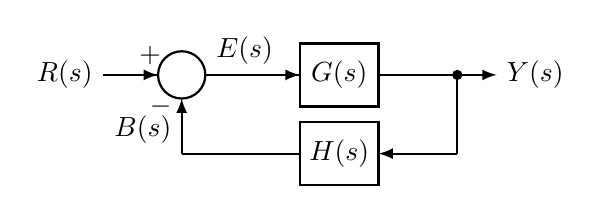
\begin{tikzpicture}[thick]
        \draw[-latex]     (2,2) -- (7,2);
        \draw[fill=white] (3,2) circle [radius=0.3];
        \draw[fill=white] (4.5,1.6) rectangle (5.5,2.4);
        \draw[fill=white] (4.5,0.6) rectangle (5.5,1.4);
        \draw[-latex]     (2,2)   -- (2.7,2);
        \draw[-latex]     (3.3,2) -- (4.5,2);
        \draw[-latex]     (6.5,1) -- (5.5,1);
        \draw[-latex]     (3,1)   -- (3,1.7);
        \draw             (6.5,2) -- (6.5,1);
        \draw             (4.5,1) -- (3,1);
        \filldraw         (6.5,2) circle [radius=0.05];
        \node[left]   at  (2,2)   {$R(s)$};
        \node[right]  at  (7,2)   {$Y(s)$};
        \node         at  (5,2)   {$G(s)$};
        \node         at  (5,1)   {$H(s)$};
        \node[above]  at  (3.8,2) {$E(s)$};
        \node[left]   at  (3,1.3) {$B(s)$};
        \node[above]  at  (2.6,2) {$+$};
        \node[left]   at  (3,1.6) {$-$};
    \end{tikzpicture}
\end{center}

闭环传递函数:

\begin{equation}
    \frac{Y(s)}{R(s)}=\frac{G(s)}{1+G(s)H(s)}
\end{equation}

前向传递函数:

\begin{equation}
    \frac{Y(s)}{E(s)}=G(s)
\end{equation}

开环传递函数:

\begin{equation}
    \frac{B(s)}{E(s)}=G(s)H(s)
\end{equation}

\section{控制系统的时域分析}

\subsection{线性定常系统}

线性定常系统的一个特性:系统对输入信号导数的响应,等于系统对该输入信号响应的导数;或者,系统对输入信号积分的响应,等于系统对该输入信号响应的积分,积分常数由零初始条件确定。

\subsection{状态空间方程的解}

系统状态空间方程为:

\begin{equation}
    \begin{aligned}
        \bm{\dot{x}}(t)&=\bm{Ax}(t)+\bm{Bu}(t) \\
        \bm{y}(t)&=\bm{Cx}(t)+\bm{Du}(t)
    \end{aligned}
\end{equation}

状态转移矩阵:

\begin{equation}
    \bm{\varPhi}(t)=\text{e}^{\bm{A}t}=\mathcal{L}^{-1}\left[(s\bm{I}-\bm{A})^{-1}\right]
\end{equation}

状态空间方程的解:

\begin{equation}
    \bm{x}(t)=\bm{\varPhi}(t)\bm{x}_0+\int_{0}^{t}\bm{\varPhi}(t-\tau)\bm{Bu}(\tau)\text{d}\tau
\end{equation}

系统的输出:

\begin{equation}
    y(t)=\bm{C\varPhi}(t)\bm{x}_0+\int_{0}^{t}\bm{C\varPhi}(t-\tau)\bm{Bu}(\tau)\text{d}\tau+\bm{Du}(t)
\end{equation}

单位阶跃响应:

\begin{equation}
    h(t)=-\bm{C}\bm{A}^{-1}\bm{B}+\bm{C}\bm{A}^{-1}\text{e}^{\bm{A}t}\bm{B}+\bm{D}
\end{equation}

静态放大系数:

\begin{equation}
    k_s=-\bm{C}\bm{A}^{-1}\bm{B}+\bm{D}
\end{equation}

\subsection{暂态性能指标}

\textbf{延迟时间}$T_d$:系统响应从0上升到稳态值的50\%所需要的时间

\textbf{上升时间}$T_r$:有振荡系统响应从0上升到稳态值所需时间;无振荡系统响应从稳态值的10\%上升到90\%所需时间。

\textbf{峰值时间}$T_p$:系统响应达到最大峰值所需要的时间。

\textbf{最大超调量}$\sigma\%$:系统响应超出稳态值的最大偏离量,常以百分比表示。

\textbf{调节时间}$T_s$:系统响应与稳态值之差达到误差$\pm\Delta$所需要的最小时间。

\textbf{振荡次数}$N$:调节时间$T_s$内,$y(t)$偏离$y(\infty)$的振荡次数。

\subsection{一阶系统的暂态响应特性}

一阶系统的闭环传递函数为:

\begin{equation}
    \frac{Y(s)}{R(s)}=\frac{1}{Ts+1}
\end{equation}

其单位阶跃响应如下:

\begin{figure}[htbp]
    \centering
    % This file was created by matlab2tikz.
%
%The latest updates can be retrieved from
%  http://www.mathworks.com/matlabcentral/fileexchange/22022-matlab2tikz-matlab2tikz
%where you can also make suggestions and rate matlab2tikz.
%
\definecolor{mycolor1}{rgb}{0.00000,0.44700,0.74100}%
%
\begin{tikzpicture}[scale=0.5]

\begin{axis}[%
width=4.396in,
height=3.357in,
at={(0.883in,0.481in)},
scale only axis,
separate axis lines,
every outer x axis line/.append style={white!40!black},
every x tick label/.append style={font=\color{white!40!black},scale=2},
every x tick/.append style={white!40!black},
xmin=0,
xmax=5,
xtick={0,1,2,3,4,5},
xticklabels={{$0$},{$T$},{$2T$},{$3T$},{$4T$},{$5T$}},
every outer y axis line/.append style={white!40!black},
every y tick label/.append style={font=\color{white!40!black},scale=2},
every y tick/.append style={white!40!black},
ymin=0,
ymax=1,
axis background/.style={fill=white},
xmajorgrids,
ymajorgrids
]
\addplot [color=mycolor1, forget plot]
  table[row sep=crcr]{%
0	0\\
0.0460517018598707	0.0450074139785543\\
0.0921034037197414	0.0879891606440716\\
0.138155105579612	0.129036410043893\\
0.184206807439483	0.168236228897295\\
0.230258509299353	0.205671765275678\\
0.276310211159224	0.24142242497077\\
0.322361913019095	0.275564039924958\\
0.368413614878966	0.308169029081007\\
0.414465316738836	0.339306551992343\\
0.460517018598707	0.369042655519742\\
0.506568720458578	0.397440413925574\\
0.552620422318448	0.424560062662772\\
0.598672124178319	0.450459126142302\\
0.64472382603819	0.475192539750152\\
0.69077552789806	0.498812766372651\\
0.736827229757931	0.521369907677283\\
0.782878931617802	0.542911810385045\\
0.828930633477672	0.563484167759754\\
0.874982335337543	0.583130616529583\\
0.921034037197414	0.601892829446421\\
0.967085739057285	0.619810603679357\\
1.01313744091716	0.636921945229817\\
1.05918914277703	0.653263149547387\\
1.1052408446369	0.668868878517327\\
1.15129254649677	0.683772233983081\\
1.19734424835664	0.698004827959718\\
1.24339595021651	0.711596849687259\\
1.28944765207638	0.724577129666104\\
1.33549935393625	0.736973200810383\\
1.38155105579612	0.748811356848964\\
1.42760275765599	0.760116708097974\\
1.47365445951586	0.770913234723147\\
1.51970616137573	0.78122383760497\\
1.5657578632356	0.791070386914523\\
1.61180956509547	0.80047376850304\\
1.65786126695534	0.809453928203605\\
1.70391296881522	0.818029914138932\\
1.74996467067509	0.826219917124994\\
1.79601637253496	0.834041309256177\\
1.84206807439483	0.841510680753823\\
1.8881197762547	0.848643875156315\\
1.93417147811457	0.855456022925345\\
1.98022317997444	0.86196157353965\\
2.02627488183431	0.868174326144299\\
2.07232658369418	0.874107458820525\\
2.11837828555405	0.879773556538201\\
2.16442998741392	0.885184637850256\\
2.21048168927379	0.890352180385627\\
2.25653339113366	0.895287145194857\\
2.30258509299353	0.899999999999948\\
2.34863679485341	0.904500741397806\\
2.39468849671328	0.90879891606436\\
2.44074019857315	0.912903641004344\\
2.48679190043302	0.916823622889686\\
2.53284360229289	0.920567176527526\\
2.57889530415276	0.924142242497037\\
2.62494700601263	0.927556403992458\\
2.6709987078725	0.930816902908064\\
2.71705040973237	0.933930655199199\\
2.76310211159224	0.936904265551941\\
2.80915381345211	0.939744041392526\\
2.85520551531198	0.942456006266247\\
2.90125721717185	0.945045912614201\\
2.94730891903172	0.947519253974987\\
2.9933606208916	0.949881276637238\\
3.03941232275147	0.952136990767703\\
3.08546402461134	0.95429118103848\\
3.13151572647121	0.956348416775952\\
3.17756742833108	0.958313061652936\\
3.22361913019095	0.960189282944621\\
3.26967083205082	0.961981060367915\\
3.31572253391069	0.963692194522962\\
3.36177423577056	0.96532631495472\\
3.40782593763043	0.966886887851715\\
3.4538776394903	0.968377223398291\\
3.49992934135017	0.969800482795955\\
3.54598104321004	0.97115968496871\\
3.59203274506991	0.972457712966595\\
3.63808444692978	0.973697320081024\\
3.68413614878966	0.974881135684883\\
3.73018785064953	0.976011670809784\\
3.7762395525094	0.977091323472302\\
3.82229125436927	0.978122383760485\\
3.86834295622914	0.979107038691441\\
3.91439465808901	0.980047376850293\\
3.96044635994888	0.98094539282035\\
4.00649806180875	0.981802991413883\\
4.05254976366862	0.98262199171249\\
4.09860146552849	0.983404130925608\\
4.14465316738836	0.984151068075373\\
4.19070486924823	0.984864387515623\\
4.2367565711081	0.985545602292526\\
4.28280827296797	0.986196157353957\\
4.32885997482785	0.986817432614422\\
4.37491167668772	0.987410745882045\\
4.42096337854759	0.987977355653813\\
4.46701508040746	0.988518463785019\\
4.51306678226733	0.989035218038556\\
4.5591184841272	0.989528714519479\\
4.60517018598707	0.989999999999988\\
4.65122188784694	0.990450074139774\\
4.69727358970681	0.99087989160643\\
4.74332529156668	0.991290364100429\\
4.78937699342655	0.991682362288963\\
4.83542869528642	0.992056717652747\\
4.88148039714629	0.992414224249699\\
4.92753209900616	0.992755640399241\\
4.97358380086604	0.993081690290802\\
};
\end{axis}

\end{tikzpicture}%

    \caption{一阶系统单位阶跃响应}
\end{figure}

延迟时间$T_d$:

\begin{equation}
    T_d=-T\ln{0.5}=0.69T
\end{equation}

上升时间$T_r$:

\begin{equation}
    T_r=(-T\ln{0.9})-(-T\ln{0.1})=2.20T
\end{equation}

\subsection{二阶规范系统的暂态响应特性}

二阶规范系统的闭环传递函数为:

\begin{equation}
    \frac{Y(s)}{R(s)}=\frac{\omega_n^2}{s^2+2\zeta\omega_n s+\omega_n^2}
\end{equation}

其中$\zeta$为阻尼比,$\omega_n$为无阻尼自然振荡角频率。
$\zeta$的值影响系统的响应情况如下表所示。

\begin{table}[htbp]
    \label{tab:zeta}
    \begin{center}
      \caption{$\zeta$的值对系统响应影响}
      \begin{tabular}{c|c|c|c|c|c}
        \hline
        $\bm{\zeta}$ & $\zeta<0$ & $\zeta=0$ & $0<\zeta<1$ & $\zeta=1$ & $\zeta>1$ \\
        \hline
        \textbf{状态} & 不稳定 & 无阻尼 & 欠阻尼 & 临界阻尼 & 过阻尼 \\
        \hline
        \textbf{响应} & - & 无衰减振荡 & 衰减振荡 & 无振荡 & 无振荡 \\
        \hline
      \end{tabular}
    \end{center}
\end{table}

欠阻尼或临界阻尼时:

\begin{equation}
    -p_{1,2}=-\zeta\omega_n\pm\text{j}\omega_n\sqrt{1-\zeta^2}=\sigma\pm\text{j}\omega_d
\end{equation}

其中,$\omega_d=\omega_n\sqrt{1-\zeta^2}$为阻尼自然振荡角频率,$\sigma=-\zeta\omega_n$为阻尼系数或衰减系数。

过阻尼时:

\begin{equation}
    -p_{1,2}=-\zeta\omega_n\pm\omega_n\sqrt{\zeta^2-1}
\end{equation}

峰值时间$T_p$:

\begin{equation}
    T_p=\frac{\pi}{\omega_d}=\frac{\pi}{\omega_n\sqrt{1-\zeta^2}}
\end{equation}

超调量$\sigma\%$:

\begin{equation}
    \sigma\%=\text{e}^{-\frac{\zeta\pi}{\sqrt{1-\zeta^2}}}\times 100\%
\end{equation}

上升时间$T_r$:

\begin{equation}
    T_r=\frac{\pi-\varphi}{\omega_d}=\frac{\pi-\varphi}{\omega_n\sqrt{1-\zeta^2}} \quad \varphi=\arctan{\frac{\sqrt{1-\zeta^2}}{\zeta}}
\end{equation}

调节时间$T_s(0<\zeta<0.9)$:

\begin{equation}
    T_s(2\%)=\frac{4}{\zeta\omega_n} \quad T_s(5\%)=\frac{3}{\zeta\omega_n}
\end{equation}

二阶工程最佳参数:

\begin{equation}
    \zeta=\frac{1}{\sqrt{2}} \quad \sigma\%=\text{e}^{-\pi}\times 100\%=4.3\%
\end{equation}

添加零点对原无零点规范二阶系统性能的影响:峰值时间提前、超调量增大(振荡加剧)、调节时间增长。

\subsection{控制系统的稳态误差}

开环传递函数$G(s)$中零极点的重数$N$,即串联的积分环节的个数,称为系统的类型或阶数。

单位反馈系统的误差系数与稳态误差的定义:

\begin{equation}
    K=\lim_{s\rightarrow 0}G(s)=\lim_{s\rightarrow 0}\frac{K}{s^N} \quad e_{ss}=\lim_{s\rightarrow 0}E(s)=\lim_{s\rightarrow 0}\frac{A}{1+G(s)}
\end{equation}

单位反馈系统的误差系数与稳态误差如下表:

\begin{table}[htbp]
    \label{tab:zeta}
    \begin{center}
      \caption{系统的误差系数与稳态误差}
      \begin{tabular}{c|c|c|c|c|c|c}
        \hline
        \multirow{2}*{系统的类型} & \multicolumn{3}{|c|}{误差系数} & \multicolumn{3}{|c}{稳态误差} \\
        \cline{2-7}
        ~ & $K_p$ & $K_v$ & $K_a$ & $e_{ss}=A/(1+K_p)$ & $e_{ss}=A/K_v$ & $e_{ss}=A/K_a$ \\
        \hline
        0型 & $K$ & $0$ & $0$ & $A/(1+K)$ & $\infty$ & $\infty$ \\ 
        \hline
        1型 & $\infty$ & $K$ & $0$ & $0$ & $A/K$ & $\infty$ \\ 
        \hline
        2型 & $\infty$ & $\infty$ & $K$ & $0$ & $0$ & $A/K$ \\ 
        \hline
      \end{tabular}
    \end{center}
\end{table}

分析非单位反馈系统的稳态误差时,开环传递函数等效为:

\begin{equation}
    G_k(s)=G(s)H(s)
\end{equation}

\subsection{控制系统的稳定性}

稳定系统:对于有界输入具有有界响应。

充要条件:系统传递函数的所有极点(系统矩阵的特征值)具有负实部(在$s$平面虚轴左面)。

稳定性判据:Routh-Hurwitz稳定性判据。

系统稳定的必要条件:特征方程的各项系数均为正(同号且不缺项)。

系统稳定的充分必要条件:Routh表中第一列各值为正。

\section{根轨迹法}

\subsection{根轨迹的基本概念}

反馈控制系统的闭环传函:

\begin{equation}
    T(s)=\frac{Y(s)}{R(s)}=\frac{G(s)}{1+G(s)H(s)}
\end{equation}

特征方程:

\begin{equation}
    1+G(s)H(s)=0
\end{equation}

开环传递函数:

\begin{equation}
    G(s)H(s)=K_g\frac{P(s)}{Q(s)}=K_g\frac{\prod\limits_{i=1}^{m}(s+z_{oi})}{\prod\limits_{j=1}^{n}(s+p_{oj})}
\end{equation}

其中$K_g$为传递系数或开环根轨迹增益,$-z_{oi}$为开环传递函数的零点,$-p_{oj}$为开环传递函数的极点。

幅角条件与幅值条件:

\begin{equation}
    \begin{aligned}
        \angle{G(s)H(s)}&=\sum_{i=1}^{m}\angle{(s+z_{oi})}-\sum_{j=1}^{n}\angle{(s+p_{oj})}=\pm(2k+1)180{^\circ}, k\in\mathbb{N} \\
        |G(s)H(s)|&=1
    \end{aligned}
\end{equation}

满足幅角条件和幅值条件的$s$值就是特征方程的根,即闭环极点。幅角条件和幅值条件构成根轨迹的基本条件。

在分析和绘制根轨迹时,幅角和幅值应可进行图解测量,故横坐标和纵坐标采用同样的尺度等分。

\subsection{绘制根轨迹的基本规则}

\textbf{规则1}:根轨迹是连续的,且对称于实轴。

\textbf{规则2}:根轨迹起始于开环极点,终止于开环零点;根轨迹的分支数(条数)为开环有限极点数和开环有限零点数中的较大值。

\textbf{规则3}:实轴上根轨迹段存在的区间的右侧,开环零点和开环极点之和为奇数。

\textbf{规则4}:根轨迹的渐近线。根轨迹有$|n-m|$条分支沿渐近线趋于或始于无穷远,这些渐近线的倾角$\phi_A$及与实轴的交点$\sigma_A$分别为:

\begin{equation}
    \begin{aligned}
        \phi_A&=\frac{2k+1}{n-m}\pi, 0\leq k\leq |n-m|-1 \\
        \sigma_A&=\frac{\sum\limits_{j=1}^{n}(-p_{oj})-\sum\limits_{i=1}^{m}(-z_{oi})}{n-m}
    \end{aligned}
\end{equation}

\textbf{规则5}:根轨迹的分离点,可由下式给出:

\begin{equation}
    \left\{
        \begin{array}{l}
            P'(s)Q(s)-Q'(s)P(s)=0 \\
            K_g\geq 0
        \end{array}
    \right.
\end{equation}

\textbf{规则6}:根轨迹与虚轴的交点为闭环系统的临界稳定点。确定与虚轴交点和临界增益值的方法:利用Routh判据,确定临界稳定点;或在特征方程中,代入$s=\mathrm{j}\omega$,令实部和虚部分别等于0,解出与虚轴交点$±\omega$和临界增益值。

\textbf{规则7}:根轨迹的出射角和入射角。

根轨迹以开环复极点$-p_{ol}$出发的出射角为:

\begin{equation}
    \theta_{p_{ol}}=\sum_{i=1}^{m}\angle[(-p_{ol})-(-z_{oi})]-\sum_{j=1,j\neq l}^{n}\angle[(-p_{ol})-(-p_{oj})]\pm 180^{\circ}(2k+1)
\end{equation}

根轨迹以开环复零点$-z_{ol}$出发的入射角为:

\begin{equation}
    \theta_{z_{ol}}=\sum_{j=1}^{n}\angle[(-z_{ol})-(-p_{oj})]-\sum_{i=1,i\neq l}^{m}\angle[(-z_{ol})-(-z_{oi})]\pm 180^{\circ}(2k+1)
\end{equation}

\textbf{规则8}:根轨迹的平衡性(走向)。当$n-m\geq 2$时,闭环极点之和为常数。因而,随着$K_g$的增大,一些根轨迹分支左行时,必有根轨迹另一些右行。

\subsection{参数根轨迹}

当以参数$X$为变量,$0\leq X<\infty$,作根轨迹时,需要将特征方程写成:

\begin{equation}
    A(s)+XB(s)=0 \quad 1+X\frac{B(s)}{A(s)}=0 \quad X\frac{B(s)}{A(s)}=-1
\end{equation}

即可同上述规则作出以$X$为变量的特征方程的根轨迹。

\subsection{绘制根轨迹举例}

\textbf{例1}

对以下开环传递函数,画出当$0<K<\infty$时的根轨迹。

\begin{equation}
    G(s)H(s)=\frac{K}{(s^2+2s+2)(s+2)}
\end{equation}

此题先绘制出零极点,并画出左侧极点的根轨迹。根据形状判断始于两个共轭极点的根轨迹是向右并趋近与渐近线。计算渐近线倾角为$\pm\dfrac{\pi}{3},\pi$和渐近线与实轴交点$\left(-\dfrac{4}{3},0\right)$。再计算一下与虚轴交点为$\left(0,\pm\mathrm{j}\sqrt{6}\right)$。粗略画出根轨迹图像,并将以上参数标注上即可(下图没有标注箭头和参数,需要自己标一下)。

\begin{figure}[htbp]
    \centering
    % This file was created by matlab2tikz.
%
%The latest updates can be retrieved from
%  http://www.mathworks.com/matlabcentral/fileexchange/22022-matlab2tikz-matlab2tikz
%where you can also make suggestions and rate matlab2tikz.
%
\definecolor{mycolor1}{rgb}{0.00000,0.44700,0.74100}%
%
\begin{tikzpicture}[scale=0.5]

\begin{axis}[%
width=4.396in,
height=3.357in,
at={(0.883in,0.481in)},
scale only axis,
unbounded coords=jump,
separate axis lines,
every outer x axis line/.append style={white!40!black},
every x tick label/.append style={font=\color{white!40!black}},
every x tick/.append style={white!40!black},
xmin=-6.14452039054368,
xmax=2,
every outer y axis line/.append style={white!40!black},
every y tick label/.append style={font=\color{white!40!black}},
every y tick/.append style={white!40!black},
ymin=-5,
ymax=5,
axis background/.style={fill=white}
]
\addplot [color=white, forget plot]
  table[row sep=crcr]{%
0	0\\
};
\addplot [color=mycolor1, only marks, mark=x, mark options={solid, mycolor1}, forget plot]
  table[row sep=crcr]{%
-2	0\\
-0.999999999999999	1\\
-0.999999999999999	-1\\
};
\addplot [color=blue, forget plot]
  table[row sep=crcr]{%
-2	0\\
-2.14230758414022	0\\
-2.1596891659192	0\\
-2.17888077068877	0\\
-2.20000774973151	0\\
-2.22319378299331	0\\
-2.24855960013578	0\\
-2.27622187450519	0\\
-2.30629236580281	0\\
-2.33887737147307	0\\
-2.3740775242599	0\\
-2.41198794683989	0\\
-2.45269874745103	0\\
-2.49629581652363	0\\
-2.54286186631368	0\\
-2.59247764507978	0\\
-2.64522325472102	0\\
-2.70117950508298	0\\
-2.76042924760164	0\\
-2.8230586434933	0\\
-2.88915833529258	0\\
-2.95882450354327	0\\
-3.03215980173525	0\\
-3.10927417155398	0\\
-3.19028554701647	0\\
-3.2753204602716	0\\
-3.36451456409525	0\\
-3.45801308684155	0\\
-3.55597123524929	0\\
-3.65855455942753	0\\
-3.76593929286511	0\\
-3.87831267865919	0\\
-3.9958732915012	0\\
-4.11883136339965	0\\
-4.24740911971976	0\\
-4.38184113090639	0\\
-4.52237468423515	0\\
-4.66927017909823	0\\
-4.8228015486594	0\\
-4.98325671018691	0\\
-5.15093804597215	0\\
-5.32616291644539	0\\
-5.5092642068902	0\\
-5.70059090901701	0\\
-5.9005087385734	0\\
-6.10940079012774	0\\
-6.32766823015954	0\\
-6.55573102961229	0\\
-6.79402873710983	0\\
-7.04302129409814	0\\
-7.30318989324969	0\\
};
\addplot [color=red, forget plot]
  table[row sep=crcr]{%
-0.999999999999999	-1\\
-0.928846207929893	-1.07586995985485\\
-0.920155417040403	-1.08573230503802\\
-0.910559614655613	-1.09675864176236\\
-0.899996125134246	-1.10905819265537\\
-0.888403108503348	-1.12274457539035\\
-0.875720199932112	-1.13793497452645\\
-0.861889062747405	-1.15474922276292\\
-0.846853817098594	-1.1733088365024\\
-0.830561314263466	-1.19373605798997\\
-0.812961237870047	-1.21615295907925\\
-0.794006026580051	-1.24068065919313\\
-0.773650626274489	-1.2674387024266\\
-0.751852091738185	-1.2965446269403\\
-0.728569066843161	-1.32811374540619\\
-0.703761177460112	-1.36225914018561\\
-0.677388372639491	-1.39909186297598\\
-0.649410247458508	-1.43872131729682\\
-0.619785376199182	-1.48125579426972\\
-0.588470678253349	-1.5268031279327\\
-0.555420832353711	-1.57547143554168\\
-0.520587748228366	-1.62736991031219\\
-0.483920099132374	-1.68260963802478\\
-0.44536291422301	-1.74130441402747\\
-0.404857226491767	-1.80357154268792\\
-0.362339769864201	-1.86953260671274\\
-0.317742717952374	-1.9393141985806\\
-0.270993456579226	-2.01304861041467\\
-0.222014382375355	-2.09087448187156\\
-0.170722720286233	-2.17293740806677\\
-0.117030353567449	-2.25939051127263\\
-0.0608436606704079	-2.35039498122508\\
-0.00206335424940263	-2.4461205894839\\
0.0594156816998229	-2.54674618352402\\
0.123704559859877	-2.65246016619843\\
0.190920565453191	-2.76346096599254\\
0.261187342117573	-2.87995750315658\\
0.334635089549114	-3.00216965640944\\
0.411400774329698	-3.13032873449336\\
0.491628355093454	-3.26467795645195\\
0.575469022986069	-3.40547294412071\\
0.6630814582227	-3.55298222997214\\
0.754632103445099	-3.70748778315057\\
0.850295454508503	-3.86928555626765\\
0.950254369286696	-4.03868605530796\\
1.05470039506387	-4.21601493481161\\
1.16383411507977	-4.40161362035659\\
1.27786551480615	-4.59583996025117\\
1.39701436855491	-4.79906890826605\\
1.52151064704907	-5.01169323918011\\
1.65159494662484	-5.23412429888219\\
};
\addplot [color=black!50!green, forget plot]
  table[row sep=crcr]{%
-0.999999999999999	1\\
-0.928846207929893	1.07586995985485\\
-0.920155417040403	1.08573230503802\\
-0.910559614655613	1.09675864176236\\
-0.899996125134246	1.10905819265537\\
-0.888403108503348	1.12274457539035\\
-0.875720199932112	1.13793497452645\\
-0.861889062747405	1.15474922276292\\
-0.846853817098594	1.1733088365024\\
-0.830561314263466	1.19373605798997\\
-0.812961237870047	1.21615295907925\\
-0.794006026580051	1.24068065919313\\
-0.773650626274489	1.2674387024266\\
-0.751852091738185	1.2965446269403\\
-0.728569066843161	1.32811374540619\\
-0.703761177460112	1.36225914018561\\
-0.677388372639491	1.39909186297598\\
-0.649410247458508	1.43872131729682\\
-0.619785376199182	1.48125579426972\\
-0.588470678253349	1.5268031279327\\
-0.555420832353711	1.57547143554168\\
-0.520587748228366	1.62736991031219\\
-0.483920099132374	1.68260963802478\\
-0.44536291422301	1.74130441402747\\
-0.404857226491767	1.80357154268792\\
-0.362339769864201	1.86953260671274\\
-0.317742717952374	1.9393141985806\\
-0.270993456579226	2.01304861041467\\
-0.222014382375355	2.09087448187156\\
-0.170722720286233	2.17293740806677\\
-0.117030353567449	2.25939051127263\\
-0.0608436606704079	2.35039498122508\\
-0.00206335424940263	2.4461205894839\\
0.0594156816998229	2.54674618352402\\
0.123704559859877	2.65246016619843\\
0.190920565453191	2.76346096599254\\
0.261187342117573	2.87995750315658\\
0.334635089549114	3.00216965640944\\
0.411400774329698	3.13032873449336\\
0.491628355093454	3.26467795645195\\
0.575469022986069	3.40547294412071\\
0.6630814582227	3.55298222997214\\
0.754632103445099	3.70748778315057\\
0.850295454508503	3.86928555626765\\
0.950254369286696	4.03868605530796\\
1.05470039506387	4.21601493481161\\
1.16383411507977	4.40161362035659\\
1.27786551480615	4.59583996025117\\
1.39701436855491	4.79906890826605\\
1.52151064704907	5.01169323918011\\
1.65159494662484	5.23412429888219\\
};
\end{axis}

\end{tikzpicture}%

    \caption{例1根轨迹图}
\end{figure}

\textbf{例2}

对以下开环传递函数,画出当$0<K<\infty$时的根轨迹。

\begin{equation}
    G(s)H(s)=\frac{K(s^2+4s+8)}{s^2(s+4)}
\end{equation}

此题先绘制出零极点,并画出左侧极点的根轨迹。根据形状判断终于两个共轭零点的根轨迹始于圆点处的极点。计算原点处极点的出射角为$\pm\dfrac{\pi}{2}$,共轭零点的入射角为$\pm\dfrac{\pi}{4}$。与虚轴交点为$(0,0)$。粗略画出根轨迹图像,并将以上参数标注上即可(下图没有标注箭头和参数,需要自己标一下)。

\begin{figure}[htbp]
    \centering
    % This file was created by matlab2tikz.
%
%The latest updates can be retrieved from
%  http://www.mathworks.com/matlabcentral/fileexchange/22022-matlab2tikz-matlab2tikz
%where you can also make suggestions and rate matlab2tikz.
%
\definecolor{mycolor1}{rgb}{0.00000,0.44700,0.74100}%
%
\begin{tikzpicture}[scale=0.5]

\begin{axis}[%
width=4.396in,
height=3.357in,
at={(0.883in,0.481in)},
scale only axis,
unbounded coords=jump,
separate axis lines,
every outer x axis line/.append style={white!40!black},
every x tick label/.append style={font=\color{white!40!black}},
every x tick/.append style={white!40!black},
xmin=-8,
xmax=2,
every outer y axis line/.append style={white!40!black},
every y tick label/.append style={font=\color{white!40!black}},
every y tick/.append style={white!40!black},
ymin=-2.5,
ymax=2.5,
axis background/.style={fill=white}
]
\addplot [color=white, forget plot]
  table[row sep=crcr]{%
0	0\\
};
\addplot [color=mycolor1, only marks, mark=o, mark options={solid, mycolor1}, forget plot]
  table[row sep=crcr]{%
-2	2\\
-2	-2\\
};
\addplot [color=mycolor1, only marks, mark=x, mark options={solid, mycolor1}, forget plot]
  table[row sep=crcr]{%
0	0\\
0	0\\
-4	0\\
};
\addplot [color=blue, forget plot]
  table[row sep=crcr]{%
0	0\\
-1.24687503881798e-05	0.00998745341739373\\
-1.62471073950383e-05	0.0114006815294031\\
-2.11704052517144e-05	0.0130138772516646\\
-2.75855909369365e-05	0.0148553331418463\\
-3.5944745424157e-05	0.0169573436438291\\
-4.68369420266298e-05	0.0193567706017398\\
-6.10297586525871e-05	0.0220956884249563\\
-7.95233693540792e-05	0.0252221199944131\\
-0.00010362102702314	0.0287908758819296\\
-0.000135020904172949	0.0328645111024753\\
-0.00017593576384625	0.0375144154370362\\
-0.000229248893873797	0.0428220553440618\\
-0.000298717293149806	0.048880387597329\\
-0.00038923642835661	0.055795466998803\\
-0.000507185218229916	0.0636882727280435\\
-0.000660875555603365	0.0726967799544854\\
-0.000861138043138941	0.0829783050110567\\
-0.00112208521513171	0.0947121533203048\\
-0.00146210601965682	0.108102598776948\\
-0.00190516161987572	0.123382220503727\\
-0.00248247377990564	0.140815616416289\\
-0.00323472470559009	0.160703500762047\\
-0.00421492311929647	0.183387171611144\\
-0.00549213800354661	0.209253299543225\\
-0.00715636194715281	0.238738933678264\\
-0.00932484421461013	0.272336535796713\\
-0.0121503341346049	0.310598723189707\\
-0.0158318032771559	0.354142205455564\\
-0.0206283749349665	0.403650110539855\\
-0.0268773838804665	0.459871470224\\
-0.0350177128458251	0.523616019270457\\
-0.0456197806117693	0.595741580761601\\
-0.0594237244223729	0.677130065041231\\
-0.0773872741884547	0.768646377523012\\
-0.100744231556621	0.871072164388362\\
-0.131072685296784	0.985003174638915\\
-0.170367849506448	1.11069501140123\\
-0.22110537977064	1.24783747609555\\
-0.286263185116448	1.39523410132859\\
-0.369236834567988	1.55036603124554\\
-0.4735282639486	1.70884317651008\\
-0.602010664839138	1.8638280446143\\
-0.755522757932933	2.00573258851601\\
-0.930724915965784	2.12290228328391\\
-1.0299264656708	2.17130027527421\\
-1.11800727604028	2.20436266182528\\
-1.30184474185039	2.24479003285775\\
-1.39259964443559	2.25068215205561\\
-1.46591183898943	2.24851065316102\\
-1.60020742178702	2.22761677052298\\
-1.70354316669372	2.19528928444422\\
-1.78038721707253	2.16087704664023\\
-1.83039369767449	2.13312511891224\\
-1.99261784563568	2.00730110547393\\
-2	2\\
};
\addplot [color=red, forget plot]
  table[row sep=crcr]{%
-4	0\\
-4.00002493750078	0\\
-4.00003249421479	0\\
-4.00004234081051	0\\
-4.00005517118189	0\\
-4.0000718894909	0\\
-4.00009367388416	0\\
-4.00012205951753	0\\
-4.00015904673922	0\\
-4.00020724205516	0\\
-4.00027004181081	0\\
-4.00035187153314	0\\
-4.00045849779979	0\\
-4.00059743461295	0\\
-4.00077847291566	0\\
-4.00101437056686	0\\
-4.00132175139966	0\\
-4.00172227672432	0\\
-4.00224417184147	0\\
-4.00292421516038	0\\
-4.00381033014168	0\\
-4.0049649628207	0\\
-4.00646948314876	0\\
-4.00842992080616	0\\
-4.01098444076969	0\\
-4.01431308781102	0\\
-4.01865049182775	0\\
-4.02430244075439	0\\
-4.03166751384472	0\\
-4.04126535399484	0\\
-4.0537736887603	0\\
-4.07007696141843	0\\
-4.09133053842081	0\\
-4.11904615907701	0\\
-4.15520703568464	0\\
-4.2024256365414	0\\
-4.2641652500639	0\\
-4.34506078507541	0\\
-4.45139996980399	0\\
-4.59187174805516	0\\
-4.77876748895323	0\\
-5.02994832606496	0\\
-5.37206762740768	0\\
-5.84566567354798	0\\
-6.51243251329682	0\\
-6.97672970435617	0\\
-7.4632683740866	0\\
-8.82262501420423	0\\
-9.76629882999878	0\\
-10.744858061856	0\\
-13.4085541841273	0\\
-17.0227296113751	0\\
-21.8477048305538	0\\
-27.2908911788489	0\\
};
\addplot [color=black!50!green, forget plot]
  table[row sep=crcr]{%
0	0\\
-1.24687503881798e-05	-0.00998745341739373\\
-1.62471073950383e-05	-0.0114006815294031\\
-2.11704052517144e-05	-0.0130138772516646\\
-2.75855909369365e-05	-0.0148553331418463\\
-3.5944745424157e-05	-0.0169573436438291\\
-4.68369420266298e-05	-0.0193567706017398\\
-6.10297586525871e-05	-0.0220956884249563\\
-7.95233693540792e-05	-0.0252221199944131\\
-0.00010362102702314	-0.0287908758819296\\
-0.000135020904172949	-0.0328645111024753\\
-0.00017593576384625	-0.0375144154370362\\
-0.000229248893873797	-0.0428220553440618\\
-0.000298717293149806	-0.048880387597329\\
-0.00038923642835661	-0.055795466998803\\
-0.000507185218229916	-0.0636882727280435\\
-0.000660875555603365	-0.0726967799544854\\
-0.000861138043138941	-0.0829783050110567\\
-0.00112208521513171	-0.0947121533203048\\
-0.00146210601965682	-0.108102598776948\\
-0.00190516161987572	-0.123382220503727\\
-0.00248247377990564	-0.140815616416289\\
-0.00323472470559009	-0.160703500762047\\
-0.00421492311929647	-0.183387171611144\\
-0.00549213800354661	-0.209253299543225\\
-0.00715636194715281	-0.238738933678264\\
-0.00932484421461013	-0.272336535796713\\
-0.0121503341346049	-0.310598723189707\\
-0.0158318032771559	-0.354142205455564\\
-0.0206283749349665	-0.403650110539855\\
-0.0268773838804665	-0.459871470224\\
-0.0350177128458251	-0.523616019270457\\
-0.0456197806117693	-0.595741580761601\\
-0.0594237244223729	-0.677130065041231\\
-0.0773872741884547	-0.768646377523012\\
-0.100744231556621	-0.871072164388362\\
-0.131072685296784	-0.985003174638915\\
-0.170367849506448	-1.11069501140123\\
-0.22110537977064	-1.24783747609555\\
-0.286263185116448	-1.39523410132859\\
-0.369236834567988	-1.55036603124554\\
-0.4735282639486	-1.70884317651008\\
-0.602010664839138	-1.8638280446143\\
-0.755522757932933	-2.00573258851601\\
-0.930724915965784	-2.12290228328391\\
-1.0299264656708	-2.17130027527421\\
-1.11800727604028	-2.20436266182528\\
-1.30184474185039	-2.24479003285775\\
-1.39259964443559	-2.25068215205561\\
-1.46591183898943	-2.24851065316102\\
-1.60020742178702	-2.22761677052298\\
-1.70354316669372	-2.19528928444422\\
-1.78038721707253	-2.16087704664023\\
-1.83039369767449	-2.13312511891224\\
-1.99261784563568	-2.00730110547393\\
-2	-2\\
};
\end{axis}

\end{tikzpicture}%

    \caption{例2根轨迹图}
\end{figure}

\section{频率响应法}

\subsection{频率特性}

频率响应:系统对正弦输入信号的稳态响应
频率特性:频率响应特性,即正弦信号输入时,系统稳态输出与输入量之比。

工程上应用最广泛的频率特性图是Bode图(对数坐标图)和极坐标图(Nyquist图、幅相频率特性图)。

极坐标图:图中反映出的量为频率特性的幅值和相角,而频率$\omega$为隐含变量。

Bode图:将频率特性分为幅频特性和相频特性,分别绘于半对数坐标上。

\subsection{典型环节的频率特性}

\subsubsection{比例环节}

\begin{equation}
    G(\mathrm{j}\omega)=K, \quad 
    \left\{
        \begin{array}{l}
            20\lg{A(\omega)}=20\lg{K} \\
            \varphi(\omega)=0
        \end{array}
    \right.
\end{equation}

\subsubsection{积分环节}

\begin{equation}
    G(\mathrm{j}\omega)=\frac{1}{\mathrm{j}\omega}, \quad 
    \left\{
        \begin{array}{l}
            20\lg{A(\omega)}=-20\lg{\omega} \\
            \varphi(\omega)=-90^{\circ}
        \end{array}
    \right.
\end{equation}

\subsubsection{微分环节}

微分环节与积分环节的Bode图关于横轴对称。

\begin{equation}
    G(\mathrm{j}\omega)=\mathrm{j}\omega, \quad 
    \left\{
        \begin{array}{l}
            20\lg{A(\omega)}=20\lg{\omega} \\
            \varphi(\omega)=90^{\circ}
        \end{array}
    \right.
\end{equation}

\subsubsection{惯性环节}

\begin{equation}
    G(\mathrm{j}\omega)=\frac{1}{1+\mathrm{j}\omega T}, \quad 
    \left\{
        \begin{array}{l}
            20\lg{A(\omega)}\approx\left\{
                \begin{array}{ll}
                    0 & \omega<\frac{1}{T} \\
                    -20\lg{\omega} & \omega>\frac{1}{T}
                \end{array}
            \right. \\
            \varphi(\omega)\approx\left\{
                \begin{array}{ll}
                    -45^{\circ}/\mathrm{dec}\cdot\omega & \frac{0.1}{T}<\omega<\frac{10}{T} \\
                    0 \stackrel{-45^{\circ}}{\rightarrow} -90^{\circ} & \omega=0 \stackrel{\frac{1}{T}}{\rightarrow} \infty
                \end{array}
            \right.
        \end{array}
    \right.
\end{equation}

\subsubsection{一阶微分环节}

一阶微分环节与一阶惯性环节的Bode图关于横轴对称。

\begin{equation}
    G(\mathrm{j}\omega)=1+\mathrm{j}\omega T, \quad 
    \left\{
        \begin{array}{l}
            20\lg{A(\omega)}\approx\left\{
                \begin{array}{ll}
                    0 & \omega<\frac{1}{T} \\
                    20\lg{\omega} & \omega>\frac{1}{T}
                \end{array}
            \right. \\
            \varphi(\omega)\approx\left\{
                \begin{array}{ll}
                    45^{\circ}/\mathrm{dec}\cdot\omega & \frac{0.1}{T}<\omega<\frac{10}{T} \\
                    0 \stackrel{45^{\circ}}{\rightarrow} 90^{\circ} & \omega=0 \stackrel{\frac{1}{T}}{\rightarrow} \infty
                \end{array}
            \right.
        \end{array}
    \right.
\end{equation}

\subsubsection{振荡环节}

\begin{equation}
    G(\mathrm{j}\omega)=\frac{1}{1-\left(\dfrac{\omega}{\omega_n}\right)^2+\mathrm{j}2\zeta\left(\dfrac{\omega}{\omega_n}\right)} (0\leq \zeta\leq 1), \quad 
    \left\{
        \begin{array}{l}
            20\lg{A(\omega)}\approx\left\{
                \begin{array}{ll}
                    0 & \omega<\frac{1}{T} \\
                    -40\lg{\omega} & \omega>\frac{1}{T}
                \end{array}
            \right. \\
            \varphi(\omega)=0 \stackrel{-90^{\circ}}{\rightarrow} -180^{\circ} \quad \omega=0  \stackrel{\frac{1}{T}}{\rightarrow} \infty
        \end{array}
    \right.
\end{equation}

谐振频率$\omega_r$与谐振峰值$M_r$($0\leq\zeta\leq\sqrt{2}$):

\begin{equation}
    \omega_r=\omega_n\sqrt{1-2\zeta^2}, \quad M_r=|G(\mathrm{j}\omega_r)|=\frac{1}{2\zeta\sqrt{1-\zeta^2}}
\end{equation}

\subsubsection{二阶微分环节}

二阶微分环节与二阶振荡环节的Bode图关于横轴对称。

\begin{equation}
    G(\mathrm{j}\omega)=1-\left(\dfrac{\omega}{\omega_n}\right)^2+\mathrm{j}2\zeta\left(\dfrac{\omega}{\omega_n}\right) (0\leq \zeta\leq 1), \quad 
    \left\{
        \begin{array}{l}
            20\lg{A(\omega)}\approx\left\{
                \begin{array}{ll}
                    0 & \omega<\frac{1}{T} \\
                    40\lg{\omega} & \omega>\frac{1}{T}
                \end{array}
            \right. \\
            \varphi(\omega)=0 \stackrel{90^{\circ}}{\rightarrow} 180^{\circ} \quad \omega=0  \stackrel{\frac{1}{T}}{\rightarrow} \infty
        \end{array}
    \right.
\end{equation}

\subsection{Nyquist稳定性判据}

判断闭环系统的稳定性(不求特征根)的方法:

\begin{enumerate}
    \setlength{\itemsep}{6pt}
    \item 代数判据:适用于特征方程为代数方程的系统,不适用于时滞系统。
    \item 根轨迹法:对于时滞系统有效,但很麻烦。
    \item Nyquist判据:利用开环频率特性$G(\mathrm{j}\omega)H(\mathrm{j}\omega)$判断闭环系统稳定性的一种图解方法。
\end{enumerate}

Nyquist判据判断特征方程$1+G(s)H(s)=0$在$s$右半平面内特征根的数目,其理论基础是复变函数的映射定理(Cauchy定理)。根据映射定理,由$F$平面上$\varGamma_F$包围原点的周数,可知$s$平面上$\varGamma_s$中的零点数与极点数。

闭环系统稳定的充要条件:

\begin{equation}
    Z=0, \quad N=Z-P=-P
\end{equation}

即$s$顺时针沿$D$形围线$\varGamma_s$变化一周时,在$1+GH$平面上, $1+G(s)H(s)$的轨迹$\varGamma_F$须逆时针包围原点$P$周。

\subsection{控制系统的稳定裕量}

稳定裕量:系统相对稳定性的一种度量,反映系统离临界稳定点的“距离”。

最小相位传递函数:在s右半平面没有极点和零点,且不含时滞环节的传递函数(时滞环节是非最小相位的)。

最小相位系统:具有最小相位传递函数的系统。

稳定的最小相位系统,开环传函$G(s)H(s)$的轨迹必不包围$(-1,0)$点。频率准则中,分为相角裕量和增益裕量。

当开环频率特性的幅值等于$1$时,其相角$\varphi(\omega_c)$与$-180^{\circ}$之差称为系统的相角裕量$\gamma$:

\begin{equation}
    \gamma=\varphi(\omega_c)-(-180^{\circ})=180^{\circ}+\varphi(\omega_c), \quad \varphi(\omega_c)=\angle{G(\mathrm{j}\omega)H(\mathrm{j}\omega)}
\end{equation}

其中$\omega_c$称为幅穿频率。$\gamma>0$时称为正相角裕量,闭环系统稳定;$\gamma<0$时称为负相角裕量,闭环系统不稳定。工程上一般常取$\gamma:30^{\circ}\sim 60^{\circ}$。

当开环频率特性的相角$\varphi(\omega_g)-180^{\circ}$时,其幅值的倒数称为系统的增益裕量$g_m$:

\begin{equation}
    a=\left|\frac{1}{G(\mathrm{j}\omega_g)H(\mathrm{j}\omega_g)}\right|, \quad g_m=20\lg{(a)}=-20\lg{|G(\mathrm{j}\omega_g)H(\mathrm{j}\omega_g)|}
\end{equation}

其中$\omega_g$称为相穿频率。$a>1, g_m>0$时称为正增益裕量,闭环系统稳定;$a<1, g_m<0$时称为负增益裕量,闭环系统不稳定。

\subsection{绘制Bode图举例}

\textbf{例3}

画出以下传递函数的Bode图。

\begin{equation}
    G(s)=\frac{1}{(0.5s+1)(2s+1)}
\end{equation}

根据$G(\mathrm{j}\omega)=\dfrac{1}{(1+0.5\mathrm{j}\omega)(1+2\mathrm{j}\omega)}$,分为$\dfrac{1}{1+2\mathrm{j}\omega}$和$\dfrac{1}{1+0.5\mathrm{j}\omega}$两个环节。

$\dfrac{1}{1+2\mathrm{j}\omega}$从$\omega=0.5$开始斜率为$-20\mathrm{dB/dec}$,$\dfrac{1}{1+0.5\mathrm{j}\omega}$从$\omega=2$开始斜率为$-20\mathrm{dB/dec}$。

将所有环节相加可得:$0<\omega<0.5$时斜率为$0$,$0.5<\omega<2$时斜率为$-20\mathrm{dB/dec}$,$\omega>2$时斜率为$-40\mathrm{dB/dec}$。

粗略画出对数幅频曲线。下图为软件绘制,手工绘制时画成折线或再加上计算几个点拟合成的曲线即可。

两个环节的相位都是$0\sim -90^{\circ}$判断相频曲线为从0变化到$-180^{\circ}$。计算$\omega=0.5,2$时的相位,再多算几个点,连接成平滑曲线即可得到相频曲线。

\begin{figure}[htbp]
    \centering
    % This file was created by matlab2tikz.
%
%The latest updates can be retrieved from
%  http://www.mathworks.com/matlabcentral/fileexchange/22022-matlab2tikz-matlab2tikz
%where you can also make suggestions and rate matlab2tikz.
%
\definecolor{mycolor1}{rgb}{0.00000,0.44700,0.74100}%
%
\begin{tikzpicture}[scale=0.75]

\begin{axis}[%
width=4.396in,
height=1.713in,
at={(0.883in,2.125in)},
scale only axis,
separate axis lines,
every outer x axis line/.append style={white!40!black},
every x tick label/.append style={font=\color{white!40!black}},
every x tick/.append style={white!40!black},
xmode=log,
xmin=0.01,
xmax=100,
xtick={0.01,0.1,1,10,100},
xticklabels={\empty},
xminorticks=true,
every outer y axis line/.append style={white!40!black},
every y tick label/.append style={font=\color{white!40!black}},
every y tick/.append style={white!40!black},
ymin=-100,
ymax=0,
ylabel={Magnitude (dB)},
axis background/.style={fill=white},
xmajorgrids,
xminorgrids,
ymajorgrids
]
\addplot [color=mycolor1, forget plot]
  table[row sep=crcr]{%
0.01	-0.00184540284797652\\
0.0116895181649858	-0.00252147313320486\\
0.0136644834929533	-0.0034451369738046\\
0.0159731228006025	-0.00470699354458726\\
0.0186718109129192	-0.00643072845301777\\
0.0218264472839749	-0.0087851400745891\\
0.0255140652003129	-0.0120004882512232\\
0.0298247128621689	-0.0163906765195733\\
0.0348636522767809	-0.0223832707334535\\
0.0407539296587178	-0.0305599765702266\\
0.0476393801040134	-0.0417109499165588\\
0.0556881399094527	-0.0569071692663009\\
0.0650967523045817	-0.0775959618625188\\
0.0760949668545988	-0.105725419177704\\
0.0889513497310823	-0.143903406472557\\
0.103979841848149	-0.195595337486784\\
0.121547425007629	-0.26536048700826\\
0.142083083253392	-0.359117376720789\\
0.166088278262772	-0.484412377310575\\
0.194149194574388	-0.650640611057536\\
0.226951053669467	-0.869136537837976\\
0.26529484644319	-1.1530233491672\\
0.310116892657478	-1.51670784521575\\
0.362511704998853	-1.97496262603594\\
0.423758716060406	-2.54167163041122\\
0.495353520895917	-3.22850251804317\\
0.579044398060249	-4.04391291835687\\
0.676875000945854	-4.99286877515122\\
0.791234261898132	-6.0774019354969\\
0.924914727721733	-7.29776911800529\\
1.08118075107661	-8.65370132139512\\
1.2638482029343	-10.1451985456664\\
1.47737765259851	-11.7725297921004\\
1.72698329065943	-13.5354383420857\\
2.01876025467904	-15.4318923485516\\
2.35983346678219	-17.4569258676994\\
2.75853161762918	-19.6020812701037\\
3.22459054529639	-21.8556908960632\\
3.76939097538836	-24.2038708067943\\
4.40623642777357	-26.6318484022448\\
5.15067807616812	-29.125216882244\\
6.02089449333613	-31.6708530552767\\
7.03813555493155	-34.2574224614666\\
8.22724134170047	-36.8755299785337\\
9.61724871115296	-39.5176292357919\\
11.2421003506209	-42.1778017115573\\
13.1414736261176	-44.8514881310421\\
15.3617494667183	-47.5352230805066\\
17.9571449437164	-50.22639869469\\
20.9910372010855	-52.9230668821199\\
24.5375110663982	-55.6237803155533\\
28.6831681334201	-58.3274680164962\\
33.5292414924956	-61.0333398290619\\
39.1940677484722	-63.7408140475733\\
45.8159766905449	-66.4494631061763\\
53.556669177069	-69.1589731013344\\
62.6051657201482	-71.8691137732056\\
73.1824221907617	-74.5797163234145\\
85.5467253556568	-77.2906570663535\\
100	-80.001845402848\\
1000	-120.000018457481\\
};
\end{axis}

\begin{axis}[%
width=4.396in,
height=1.519in,
at={(0.883in,0.481in)},
scale only axis,
separate axis lines,
every outer x axis line/.append style={white!40!black},
every x tick label/.append style={font=\color{white!40!black}},
every x tick/.append style={white!40!black},
xmode=log,
xmin=0.01,
xmax=100,
xminorticks=true,
every outer y axis line/.append style={white!40!black},
every y tick label/.append style={font=\color{white!40!black}},
every y tick/.append style={white!40!black},
ymin=-181.8,
ymax=1.8,
ytick={-180, -135,  -90,  -45,    0},
ylabel={Phase (deg)},
axis background/.style={fill=white},
xmajorgrids,
xminorgrids,
ymajorgrids
]
\addplot [color=mycolor1, forget plot]
  table[row sep=crcr]{%
0.001	-0.143239293607002\\
0.01	-1.43223934845217\\
0.0116895181649858	-1.67415235392956\\
0.0136644834929533	-1.95689734096321\\
0.0159731228006025	-2.287349283216\\
0.0186718109129192	-2.67353058932355\\
0.0218264472839749	-3.12479657525627\\
0.0255140652003129	-3.65204730400385\\
0.0298247128621689	-4.26796732918776\\
0.0348636522767809	-4.9872934537518\\
0.0407539296587178	-5.82710800944547\\
0.0476393801040134	-6.8071506943233\\
0.0556881399094527	-7.95013467320115\\
0.0650967523045817	-9.28204105066036\\
0.0760949668545988	-10.8323481532194\\
0.0889513497310823	-12.6341262629967\\
0.103979841848149	-14.7238929299935\\
0.121547425007629	-17.1410792638048\\
0.142083083253392	-19.9269096676493\\
0.166088278262772	-23.1224635138134\\
0.194149194574388	-26.7657029005031\\
0.226951053669467	-30.8873738673749\\
0.26529484644319	-35.5059873668835\\
0.310116892657478	-40.6225905387416\\
0.362511704998853	-46.2166463376667\\
0.423758716060406	-52.2447285483566\\
0.495353520895917	-58.6434289553271\\
0.579044398060249	-65.3365693472751\\
0.676875000945854	-72.2448791234204\\
0.791234261898132	-79.2948212529951\\
0.924914727721733	-86.4232998258091\\
1.08118075107661	-93.5767001741909\\
1.2638482029343	-100.705178747005\\
1.47737765259851	-107.75512087658\\
1.72698329065943	-114.663430652725\\
2.01876025467904	-121.356571044673\\
2.35983346678219	-127.755271451643\\
2.75853161762918	-133.783353662333\\
3.22459054529639	-139.377409461258\\
3.76939097538836	-144.494012633117\\
4.40623642777357	-149.112626132625\\
5.15067807616812	-153.234297099497\\
6.02089449333613	-156.877536486187\\
7.03813555493155	-160.073090332351\\
8.22724134170047	-162.858920736195\\
9.61724871115296	-165.276107070006\\
11.2421003506209	-167.365873737003\\
13.1414736261176	-169.167651846781\\
15.3617494667183	-170.71795894934\\
17.9571449437164	-172.049865326799\\
20.9910372010855	-173.192849305677\\
24.5375110663982	-174.172891990555\\
28.6831681334201	-175.012706546248\\
33.5292414924956	-175.732032670812\\
39.1940677484722	-176.347952695996\\
45.8159766905449	-176.875203424744\\
53.556669177069	-177.326469410676\\
62.6051657201482	-177.712650716784\\
73.1824221907617	-178.043102659037\\
85.5467253556568	-178.32584764607\\
100	-178.567760651548\\
1000	-179.856760706393\\
};
\end{axis}

\end{tikzpicture}%

    \caption{例3 Bode图}
\end{figure}

\subsection{Nyquist稳定性判据举例}

\textbf{例4}

画出当$K=4$时的极坐标图。

\begin{equation}
    G(s)H(s)=\frac{K}{(s+1)^2}
\end{equation}

计算$D$型曲线对应的点,没有零极点需要避开:

\begin{equation}
    \begin{array}{ll}
        A: s=\infty\mathrm{e}^{-\mathrm{j}90^{\circ}} & 
        A': G(s)H(s)=\dfrac{K}{s^2}=0\mathrm{e}^{\mathrm{j}180^{\circ}} \\
        B: s=0\mathrm{e}^{-\mathrm{j}90^{\circ}} & 
        B': G(s)H(s)=K=4\mathrm{e}^{\mathrm{j}0^{\circ}} \\
        C: s=0\mathrm{e}^{\mathrm{j}90^{\circ}} & 
        C': G(s)H(s)=K=4\mathrm{e}^{\mathrm{j}0^{\circ}} \\
        D: s=\infty\mathrm{e}^{\mathrm{j}90^{\circ}} & 
        D': G(s)H(s)=\dfrac{K}{s^2}=0\mathrm{e}^{-\mathrm{j}180^{\circ}} \\
        E: s=\infty\mathrm{e}^{-\mathrm{j}0^{\circ}} & 
        E': G(s)H(s)=\dfrac{K}{s^2}=0\mathrm{e}^{\mathrm{j}0^{\circ}} \\
    \end{array}
\end{equation}

求与实轴的交点:

\begin{equation}
    v=\mathrm{Im}[G(\mathrm{j}\omega)H(\mathrm{j}\omega)]=0, \quad \omega=\pm 2
\end{equation}

根据以上计算结果粗略绘制图像:

\begin{figure}[htbp]
    \centering
    % This file was created by matlab2tikz.
%
%The latest updates can be retrieved from
%  http://www.mathworks.com/matlabcentral/fileexchange/22022-matlab2tikz-matlab2tikz
%where you can also make suggestions and rate matlab2tikz.
%
\definecolor{mycolor1}{rgb}{0.00000,0.44700,0.74100}%
%
\begin{tikzpicture}[scale=0.6]

\begin{axis}[%
width=4.396in,
height=3.357in,
at={(0.883in,0.481in)},
scale only axis,
separate axis lines,
every outer x axis line/.append style={white!40!black},
every x tick label/.append style={font=\color{white!40!black}},
every x tick/.append style={white!40!black},
xmin=-1,
xmax=4,
every outer y axis line/.append style={white!40!black},
every y tick label/.append style={font=\color{white!40!black}},
every y tick/.append style={white!40!black},
ymin=-3,
ymax=3,
axis background/.style={fill=white}
]
\addplot [color=red, mark=+, mark options={solid, red}, forget plot]
  table[row sep=crcr]{%
-1	0\\
};
\addplot [color=mycolor1, forget plot]
  table[row sep=crcr]{%
4	0\\
4	0\\
4	0\\
3.9999999952	-0.000159999999871289\\
3.99995200032	-0.0159998720007683\\
3.99520319820892	-0.15987207675906\\
3.99380166537382	-0.181708396616789\\
3.99199108778137	-0.206513142568202\\
3.98965238890689	-0.234683224524424\\
3.98663203234811	-0.2666655141843\\
3.98273218612236	-0.30296165616181\\
3.97769817121969	-0.344132602790048\\
3.97120250630326	-0.390802410534271\\
3.96282472853877	-0.443660586387437\\
3.95202604447951	-0.503461912684731\\
3.93811777392167	-0.571022167280211\\
3.92022254723994	-0.647207442098942\\
3.89722739579141	-0.732913789477369\\
3.86772838926512	-0.829032639702611\\
3.82996756659893	-0.936395812221024\\
3.78176494382324	-1.05569204745146\\
3.72045187600504	-1.18734505718346\\
3.64281764948261	-1.33134171730006\\
3.54508955299958	-1.48699939425373\\
3.42297817414036	-1.65266561378713\\
3.27183358792388	-1.82535464505058\\
3.08697135748867	-2.00034844968239\\
2.86423245460005	-2.17082802079767\\
2.60082482953701	-2.32765594091922\\
2.2964373896932	-2.45949222553381\\
1.95450230415473	-2.55346432828904\\
1.58331194937103	-2.59657642336737\\
1.19652397237461	-2.5778719713382\\
0.812528643376635	-2.49103596875047\\
0.452352722168389	-2.33672929255515\\
0.1362906991244	-2.123718727902\\
-0.119884292536309	-1.86806963994112\\
-0.307868605433279	-1.59036422976636\\
-0.427877063786139	-1.31177794750129\\
-0.487521599954386	-1.05034942630543\\
-0.499150003295307	-0.81858861154633\\
-0.47675242032657	-0.622854368675632\\
-0.433414523162592	-0.464188422874552\\
-0.379797484621742	-0.339906733197157\\
-0.32362448606441	-0.245277963189258\\
-0.269872009636166	-0.174876276314902\\
-0.221313843502936	-0.123470904432038\\
-0.179148689214565	-0.0864956956654581\\
-0.143558478298951	-0.0602160727053861\\
-0.114138247157635	-0.0417141412505366\\
-0.0901948184722905	-0.0287847754697012\\
-0.0709369579129086	-0.0198022837091899\\
-0.0555859785479883	-0.0135903180968098\\
-0.0434328430242659	-0.00930966212677563\\
-0.0338618099389565	-0.00636806245068575\\
-0.0263546512768278	-0.00435100972833658\\
-0.0204845950381327	-0.00297024074089174\\
-0.0159056203300055	-0.00202627056189767\\
-0.0123403594157172	-0.00138157286018239\\
-0.00956835123893953	-0.000941612703729139\\
-0.00741547596843435	-0.000641553716772298\\
-0.00574487311222289	-0.000437005600974908\\
-0.00444936075488059	-0.000297617403328002\\
-0.00344523346295809	-0.000202658883409134\\
-0.00266725963518234	-0.000137982314387619\\
};
\addplot [color=mycolor1, forget plot]
  table[row sep=crcr]{%
4	-0\\
4	-0\\
4	-0\\
3.9999999952	0.000159999999871289\\
3.99995200032	0.0159998720007683\\
3.99520319820892	0.15987207675906\\
3.99380166537382	0.181708396616789\\
3.99199108778137	0.206513142568202\\
3.98965238890689	0.234683224524424\\
3.98663203234811	0.2666655141843\\
3.98273218612236	0.30296165616181\\
3.97769817121969	0.344132602790048\\
3.97120250630326	0.390802410534271\\
3.96282472853877	0.443660586387437\\
3.95202604447951	0.503461912684731\\
3.93811777392167	0.571022167280211\\
3.92022254723994	0.647207442098942\\
3.89722739579141	0.732913789477369\\
3.86772838926512	0.829032639702611\\
3.82996756659893	0.936395812221024\\
3.78176494382324	1.05569204745146\\
3.72045187600504	1.18734505718346\\
3.64281764948261	1.33134171730006\\
3.54508955299958	1.48699939425373\\
3.42297817414036	1.65266561378713\\
3.27183358792388	1.82535464505058\\
3.08697135748867	2.00034844968239\\
2.86423245460005	2.17082802079767\\
2.60082482953701	2.32765594091922\\
2.2964373896932	2.45949222553381\\
1.95450230415473	2.55346432828904\\
1.58331194937103	2.59657642336737\\
1.19652397237461	2.5778719713382\\
0.812528643376635	2.49103596875047\\
0.452352722168389	2.33672929255515\\
0.1362906991244	2.123718727902\\
-0.119884292536309	1.86806963994112\\
-0.307868605433279	1.59036422976636\\
-0.427877063786139	1.31177794750129\\
-0.487521599954386	1.05034942630543\\
-0.499150003295307	0.81858861154633\\
-0.47675242032657	0.622854368675632\\
-0.433414523162592	0.464188422874552\\
-0.379797484621742	0.339906733197157\\
-0.32362448606441	0.245277963189258\\
-0.269872009636166	0.174876276314902\\
-0.221313843502936	0.123470904432038\\
-0.179148689214565	0.0864956956654581\\
-0.143558478298951	0.0602160727053861\\
-0.114138247157635	0.0417141412505366\\
-0.0901948184722905	0.0287847754697012\\
-0.0709369579129086	0.0198022837091899\\
-0.0555859785479883	0.0135903180968098\\
-0.0434328430242659	0.00930966212677563\\
-0.0338618099389565	0.00636806245068575\\
-0.0263546512768278	0.00435100972833658\\
-0.0204845950381327	0.00297024074089174\\
-0.0159056203300055	0.00202627056189767\\
-0.0123403594157172	0.00138157286018239\\
-0.00956835123893953	0.000941612703729139\\
-0.00741547596843435	0.000641553716772298\\
-0.00574487311222289	0.000437005600974908\\
-0.00444936075488059	0.000297617403328002\\
-0.00344523346295809	0.000202658883409134\\
-0.00266725963518234	0.000137982314387619\\
};

\addplot[area legend, draw=mycolor1, fill=mycolor1, forget plot]
table[row sep=crcr] {%
x	y\\
1.69139417756339	-2.65560611086886\\
1.58331194937103	-2.59657642336737\\
1.67995407092866	-2.51376892074347\\
}--cycle;

\addplot[area legend, draw=mycolor1, fill=mycolor1, forget plot]
table[row sep=crcr] {%
x	y\\
1.48666982781339	2.67938392599128\\
1.58331194937103	2.59657642336737\\
1.47522972117867	2.53754673586588\\
}--cycle;
\end{axis}

\end{tikzpicture}%

    \caption{例4 Nyquist图}
\end{figure}

\section{控制系统设计}

\subsection{常用校正环节}

\subsubsection{超前校正}

超前校正网络传递函数:

\begin{equation}
    G_c(s)=\frac{1}{\alpha}\frac{\alpha T_d s+1}{T_d s+1}=\frac{s+z_d}{s+p_d}, \quad \alpha=\frac{1+\sin{\varphi_m}}{1-\sin{\varphi_m}}>1
\end{equation}

其零极点为:

\begin{equation}
    -z_d=-\frac{1}{\alpha T_d}, \quad -p_d=-\frac{1}{T_d}
\end{equation}

最大超前相移角处的频率$\omega_m$:

\begin{equation}
    \omega_m=\frac{1}{\sqrt{\alpha}T_d}, \quad 20\lg{|G_c(\mathrm{j}\omega_m)|}=-10\lg{\alpha}
\end{equation}

\subsubsection{滞后校正}

滞后校正网络传递函数:

\begin{equation}
    G_c(s)=\frac{\beta T_i s+1}{T_i s+1}=\beta\frac{s+z_i}{s+p_i}, \quad \beta<1
\end{equation}

确定分度系数$\beta$:

\begin{equation}
    20\lg{|K_c G_o(\mathrm{j}\omega_c)|}+20\lg{\beta}=0
\end{equation}

其零极点为:

\begin{equation}
    -z_i=-\frac{1}{\beta T_i}, \quad -p_i=-\frac{1}{T_i}
\end{equation}

最大超前相移角处的频率$\omega_m$:

\begin{equation}
    \omega_m=\frac{1}{\sqrt{\beta}T_i}
\end{equation}

\subsubsection{滞后—超前校正}

滞后—超前校正网络传递函数:

\begin{equation}
    G_c(s)=\frac{\beta T_i s+1}{T_i s+1}\frac{\alpha T_d s+1}{T_d s+1}=\frac{s+z_i}{s+p_i}\frac{s+z_d}{s+p_d}, \quad \beta<1, \alpha=\frac{1}{\beta}>1,T_i>T_d
\end{equation}

\subsubsection{PID控制器}

PID控制器传递函数:

\begin{equation}
    G_c(s)=K_p+\frac{K_I}{s}+K_D s
\end{equation}

\subsection{基于频域法的串联校正}

\subsubsection{串联超前校正}

串联超前校正通过增大开环增益改善静态特征;超前校正环节转折频率选择在预定的幅穿频率的两边,提高相角裕量,改善动态特征。

\textbf{频率法串联超前校正参考步骤}

\begin{enumerate}
    \setlength{\itemsep}{6pt}
    \item 如果有要求静态误差系数指标,先根据静态误差系数确定附加增益$K_{c_1}$;
    \item 画出$K_{c_1}G_o(\mathrm{j}\omega)$的Bode图,得到$\gamma_o$和$g_{m_o}$,并根据$\omega_c$附近频率特性斜率取相角预留量$\varepsilon$,斜率为$-40\mathrm{dB/dec}$时取$5^{\circ}\sim 10^{\circ}$,斜率为$-60\mathrm{dB/dec}$时取$15^{\circ}\sim 20^{\circ}$;
    \item 计算$\varphi_m=\gamma-\gamma_0+\varepsilon$,$\alpha=\dfrac{1+\sin{\varphi_m}}{1-\sin{\varphi_m}}$;
    \item 在原频率特性曲线上通过$20\lg{|K_{c_1}G_c(\mathrm{j}\omega_m)|}=-20\lg{\sqrt{\alpha}}=-10\lg{\alpha}$确定$\omega_m$,并令新的幅穿频率$\omega_c=\omega_m$;
    \item 由$\omega_m=\dfrac{1}{\sqrt{\alpha}T_d}$计算$T_d$和$-z_d=-\dfrac{1}{\alpha T_d}, \quad -p_d=-\dfrac{1}{T_d}$;
    \item 确定补偿超前环节增益衰减应附加的增益$K_{c_2}=\alpha$,则超前环节总的附加增益$K_c=K_{c_1}K_{c_2}$;
    \item 作出校正后系统的Bode图,检查性能指标是否满足
    要求。
\end{enumerate}

\textbf{不适用串联超前校正的情况}

\begin{enumerate}
    \setlength{\itemsep}{6pt}
    \item 若需要$\varphi_m$太大时($>60^{\circ}$),串联一个超前环节难以满足要求。
    \item 若原系统$G_o(\mathrm{j}\omega)$的相频特性$\varphi_o(\omega)$在$\omega_c$附近下降太快时,超前校正往往无效。
\end{enumerate}

\subsubsection{串联滞后校正}

校正前系统在幅穿频率附近相频特性下降很快时,采用超前校正往往无效。若对校正后系统的幅穿频率要求不高,可考虑采用滞后校正。

\textbf{频率法串联滞后校正参考步骤}

\begin{enumerate}
    \setlength{\itemsep}{6pt}
    \item 如果有要求静态误差系数指标,先根据静态误差系数确定附加增益$K_{c}$;
    \item 画出$K_{c}G_o(\mathrm{j}\omega)$的Bode图,得到$\gamma_o$和$g_{m_o}$;
    \item 根据相角裕量条件$\gamma_o(\omega_c)=\gamma+|\varphi_i(\omega_c)|$,$|\varphi_i(\omega_c)|$取$5^{\circ}\sim 12^{\circ}$,在相位曲线上确定新的幅穿频率$\omega_c$;
    \item 根据$20\lg{|K_c G_o(\mathrm{j}\omega_c)|}+20\lg{\beta}=0$确定分度系数$\beta$;
    \item 选择零点对应的转折频率$\dfrac{1}{\beta T_i}$,使$|\varphi_i(\omega_c)|$不大于预留的滞后相角,一般取$\dfrac{1}{\beta T_i}=\dfrac{\omega_c}{5\sim 10}$。
    \item 作出校正后系统的Bode图,检查性能指标是否满足要求。
\end{enumerate}

\subsection{基于根轨迹法的串联校正}

性能指标以时域指标给出,如超调量、调整时间、上升时间等,以及闭环主导极点的阻尼比、无阻尼自然振荡频率等,常采用根轨迹法校正。

往往通过选择一对闭环主导极点,使校正后的系统满足性能指标。

\subsubsection{串联超前校正}

通过合理配置超前校正环节的一对零、极点,改变根轨迹的形状,以获得希望的系统根轨迹。主要用于改善动态指标。

\textbf{根轨迹法串联超前校正参考步骤}

\begin{enumerate}
    \setlength{\itemsep}{6pt}
    \item 根据动态性能指标,确定希望的闭环主导极点的预期位置;
    \item 绘制原系统的根轨迹图,验证未校正系统能否具有预期主导极点。如有,则只需调整增益值。若无,则计算要通过预期闭环极点未校正系统所需的相角缺额,即为超前校正环节应提供的超前相角$\varphi_c$;
    \item 根据$\varphi_c$,确定超前校正环节的零点和极点;
    \item 根据幅值条件$|G_c(s_1)G_o(s_1)|=1$,确定校正环节附加增益$K_c$,$G_c(s)=K_c\dfrac{s+z_d}{s+p_d}$;
    \item 检验校正后系统的性能指标:检查预期的闭环极点是否为主导极点;如是,按无零点二阶系统估算性能指标。如不能满足性能指标,则需要修正参数,直到满足要求。
\end{enumerate}

\textbf{作图法确定零极点}

\begin{enumerate}
    \setlength{\itemsep}{6pt}
    \item 过$s_1$点,作$\overline{s_1 A}$平行于负实轴;
    \item 作$\angle O s_1 A$的角平分线$\overline{s_1 B}$;
    \item 在角平分线两侧用$\pm\dfrac{\varphi_c}{2}$分别做出$\overline{s_1 C}$和$\overline{s_1 D}$;
    \item $\overline{s_1 C}$和$\overline{s_1 D}$与负实轴的交点即为的零点和极点。
\end{enumerate}

\textbf{计算法确定零极点}

\begin{enumerate}
    \setlength{\itemsep}{6pt}
    \item 计算$\delta=\dfrac{1}{2}(180^{\circ}-\varphi-\varphi_c)$;
    \item 计算零极点:$z_d=\dfrac{\sin{\delta}}{\sin{(\varphi+\delta)}}\omega$,$p_d=\dfrac{\sin{(\varphi+\delta)}}{\sin{\delta}}\omega$。
\end{enumerate}

\subsubsection{串联滞后校正}

\textbf{根轨迹法串联滞后校正参考步骤}

\begin{enumerate}
    \setlength{\itemsep}{6pt}
    \item 绘制未校正系统的根轨迹图。根据动态性能指标,在根轨迹上确定希望的闭环主导极点的位置;
    \item 计算对应于闭环主导极点的开环增益;
    \item 根据稳态误差系数的要求,计算应由校正环节提供的附加增益值$K_c$。按$K_c\beta=1$考虑选取$\beta=\dfrac{1}{K_c}$;
    \item 确定零、极点的值$\dfrac{1}{\beta T_i}$、$\dfrac{1}{T_i}$,为使滞后网络对系统动态性能不产生明显的影响,一般选取$\beta T_i$为原系统最大时间常数10倍以上;
    \item 做出校正后系统的根轨迹图,确定对应于闭环主导极点的开环增益值;
    \item 检验原设计的闭环主导极点是否满足闭环主导极点的条件。若确为闭环主导极点,即可按无零点二阶系统估算性能指标。
\end{enumerate}

\section{非线性系统分析}

\subsection{描述函数法}

在一定条件下,非线性环节在正弦信号作用下的输出,可用其一次谐波分量来近似,从而将非线性系统等效为线性系统;于是可将线性系统的频域法,推广用来分析研究非线性系统的稳定性和自持振荡问题。

描述函数也是非线性特性的一种线性化处理,称为谐波线性化。

基于平衡态附近的小信号分析的线性化仅适用于非本质非线性系统。

\subsection{非线性系统的描述函数分析}

假定非线性环节的输入输出特性是奇对称的,即直流分量为零;而且线性部分具有良好的低通滤波特性。

非线性环节的描述函数定义为在正弦输入时该环节输出的基波分量与输入信号的复数符号之比,即:

\begin{equation}
    N=\frac{y_1}{A}\mathrm{e}^{\mathrm{j}\varphi_1}=\frac{B_1}{A}+\mathrm{j}\frac{A_1}{A}
\end{equation}

其中$A$为正弦输入信号的幅值;$y_1$为输出信号基波分量的幅值;$\varphi_1$为输出信号基波分量的相移角。

非线性系统的特征方程为:

\begin{equation}
    N(A)G(s)+1=0
\end{equation}

非线性系统的频域形式为:

\begin{equation}
    G(\mathrm{j}\omega)=-N^{-1}(A)
\end{equation}

其中$-N^{-1}(A)$称为非线性特性的负倒描述函数。应用Nyquist判据,相当于线性系统中的$G(\mathrm{j}\omega)=-1$。

设非线性系统的线性部分$G(s)$是最小相位的,于是, 闭环系统稳定的条件为$N=0$。

若$G(\mathrm{j}\omega)$曲线不包围$-N^{-1}(A)$曲线,则非线性系统是稳定的;若$G(\mathrm{j}\omega)$曲线包围$-N^{-1}(A)$曲线,则非线性系统是不稳定的;若$G(\mathrm{j}\omega)$曲线与$-N^{-1}(A)$曲线相交,则非线性系统可能出现自持振荡。

\begin{figure}[htbp]
    \centering
    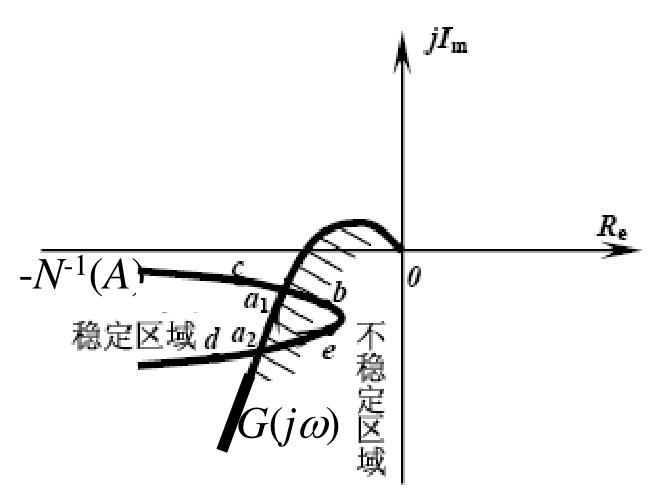
\includegraphics[width=0.4\textwidth]{Non-Liner.jpg}
    \caption{非线性控制系统的描述函数分析}
\end{figure}

在图示的非线性控制系统中,若$a_1$点产生移动向$b$点的扰动,系统会不稳定,使振幅$A$增大,工作点回到$a_1$点;若$a_1$点产生移动向$c$点的扰动,系统稳定,使振幅$A$减小,工作点回到$a_1$点。

$a_1$点具有收敛性。这说明工作点在$a_1$点时系统是稳定的,呈现稳定的自持振荡:振幅为$A_1$,频率为$\omega_1$,该自振可近似表示为$A_1\sin{\omega_1 t}$。$a_2$点具有发散性。即$a_2$点周期运动是不稳定的,无法维持。

\subsection{典型非线性特性}

\subsubsection{理想继电型特性}

负倒描述函数曲线为整个负实轴。为稳定的自持振荡。计算交点方式为令$\mathrm{Im}[G(\mathrm{j}\omega)]=0$,下同。

\subsubsection{具有死区的三位置继电型特性}

当$A=b$和$A\rightarrow \infty$时,$-N^{-1}(A)\rightarrow-\infty$;当$A=\sqrt{2}b$时,$-N^{-1}(A)$为最大值,若相交则存在一个稳定的自持振荡的点和一个不稳定的振荡的点。

\subsubsection{饱和非线性特性}

当$A\rightarrow \infty$时,$-N^{-1}(A)\rightarrow-\infty$;当$A=b$时,$-N^{-1}(A)=-\dfrac{1}{k}$为最大值,该点是稳定的自持振荡。

\subsubsection{死区非线性特性}

当$A=\Delta$时,$-N^{-1}(A)\rightarrow-\infty$;当$A\rightarrow \infty$时,$-N^{-1}(A)=-\dfrac{1}{k}$为最大值,该点是不稳定的振荡。

\subsection{相平面法}

将系统运动过程转化为在状态空间中系统状态转移的轨迹,通过绘制和研究从不同的初始状态出发的状态轨迹,获知系统运动的有关信息。相平面法通常只用于分析二阶系统。

\subsection{相平面法的基本概念}

设二阶自治系统:

\begin{equation}
    \ddot{x}=f(x,\dot{x}), \quad \frac{\mathrm{d}\dot{x}}{{\mathrm{d}x}}=\frac{f(x,\dot{x})}{\dot{x}}
\end{equation}

取$x$为横坐标,$\dot{x}$为纵坐标,构成的二维状态空间称为相平面,对应的状态轨迹称为相轨迹,而$\dfrac{\mathrm{d}\dot{x}}{\mathrm{d}x}$是相轨迹的斜率。

当$\dot{x}=0$且$\ddot{x}=f(x,\dot{x})=0$的点称为奇点,奇点处的相轨迹斜率为不定的。其他的点称为普通点。系统的平衡点是奇点。

\subsection{二阶线性系统的自由运动}

\textbf{奇点的类型}

\begin{enumerate}
    \setlength{\itemsep}{6pt}
    \item 中心点:$\zeta=0$,相轨迹为一簇围绕奇点的椭圆形封闭曲线,系统的自由运动为等幅正弦振荡。
    \item 稳定焦点:$0<\zeta<1$,相轨迹是由外向奇点趋近的一簇对数螺旋线,系统的自由运动为衰减振荡。
    \item 不稳定焦点:$-1<\zeta<0$,相轨迹是由奇点向外发散的一簇对数螺旋线,系统的自由运动为发散振荡。
    \item 稳定结点:$\zeta>1$,系统极点为两个负实根,相轨迹为由外向奇点趋近的一簇抛物线。
    \item 不稳定结点:$\zeta<-1$,系统极点为两个正实根,相轨迹为由奇点向外发散的一簇抛物线。
    \item 鞍点:系统极点为两个异号的实根时,系统的自由运动是非周期发散的。
\end{enumerate}

\begin{figure}[htbp]
    \centering
    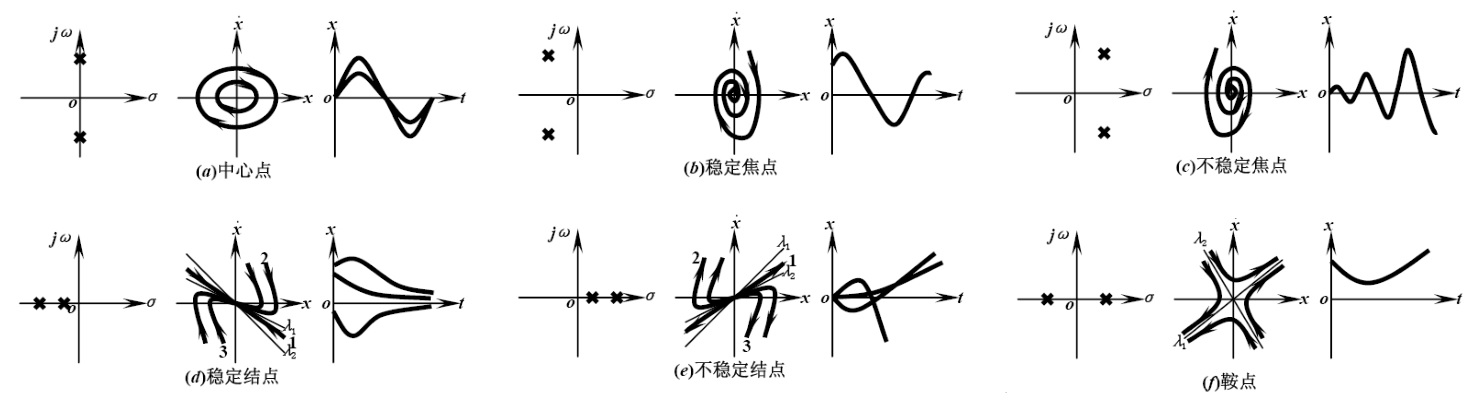
\includegraphics[width=\textwidth]{Node.jpg}
    \caption{奇点的类型}
\end{figure}

\subsubsection{由相图求系统的时间响应特性}

相轨迹图表示出系统状态变量之间的关系,时间信息隐含其中,可由相轨迹图获取时间信息。

\begin{equation}
    t_{ab}=t_b-t_a=\int_{x_a}^{x_b}\frac{1}{\dot{x}}\mathrm{d}x
\end{equation}

\textbf{积分法}

利用$\dfrac{1}{\dot{x}}$曲线计算时间。系统相轨迹为$x\sim \dot{x}$曲线,变换为$x\sim \dfrac{1}{\dot{x}}$。

在$\Delta x$区间内$\dot{x}$的值较大且变化不大时,以增量作为近似计算,即为“增量法”:

\begin{equation}
    \Delta t=\frac{1}{\dot{x}_{\mathrm{av}}\Delta x}
\end{equation}

其中$\dot{x}_{\mathrm{av}}$为区间内$\dot{x}$的平均值。

\textbf{圆弧法}

用圆心位于$x$轴上的一系列小圆弧来近似表示所研究的相轨迹段。

若角度以弧度为单位,时间以秒为单位,则在数值上等于小圆弧所对应的中心角,即:

\begin{equation}
    t_{ab}=\theta_a-\theta_b=\theta_{\wideparen{ab}}
\end{equation}

\section{MATLAB的应用}

\begin{lstlisting}[language=Matlab]
    %% 需要掌握的函数
    tf(num,den);  % 由分子多项式和分母多项式生成传递函数
    conv(a,b);    % 多项式相乘
    step(sys);    % 绘制系统阶跃响应图像
    bode(sys);    % 绘制系统波特图,包括幅频曲线和相频曲线
    pzmap(sys);   % 绘制系统零极点分布图
    rlocus(sys);  % 绘制系统根轨迹
    nyquist(sys); % 绘制系统Nyquist图,即极坐标图
    
    %% 举例
    sys=tf(1,conv([1,1,1],[2,1])); % 1/[(s^2+s+1)(2s+1)]
    rlocus(sys);
    nyquist(sys);
\end{lstlisting}

\end{document}
